
\chapter{Instancia��o}
\label{cap:instancia}


% Present the NCB instance (model) . Describe its use: how it is instantiated (i.e., put to run in the form of an execution engine) and how it interprets a user-derived model at runtime (describe the model that is seen by the NCB layer, i.e., based on the commands available at its interface with the UCM layer).
In order to demonstrate the usage of the proposed  metamodel along with the provided execution environment, we designed a model that describes the behavior present in the NCB layer of the CVM. The existing CVM implementation of NCB was analyzed and used as a reference for the construction of this model. In order to verify its accuracy we designed a set of automated test scenarios that simulate requests from the middleware layer.
These tests were executed both in the existing NCB implementation, and in the modeled NCB loaded in the execution engine, leading to same expected results. 
%[Refers to Andrew's NCB implementation] 

\begin{figure*}
 \centering
 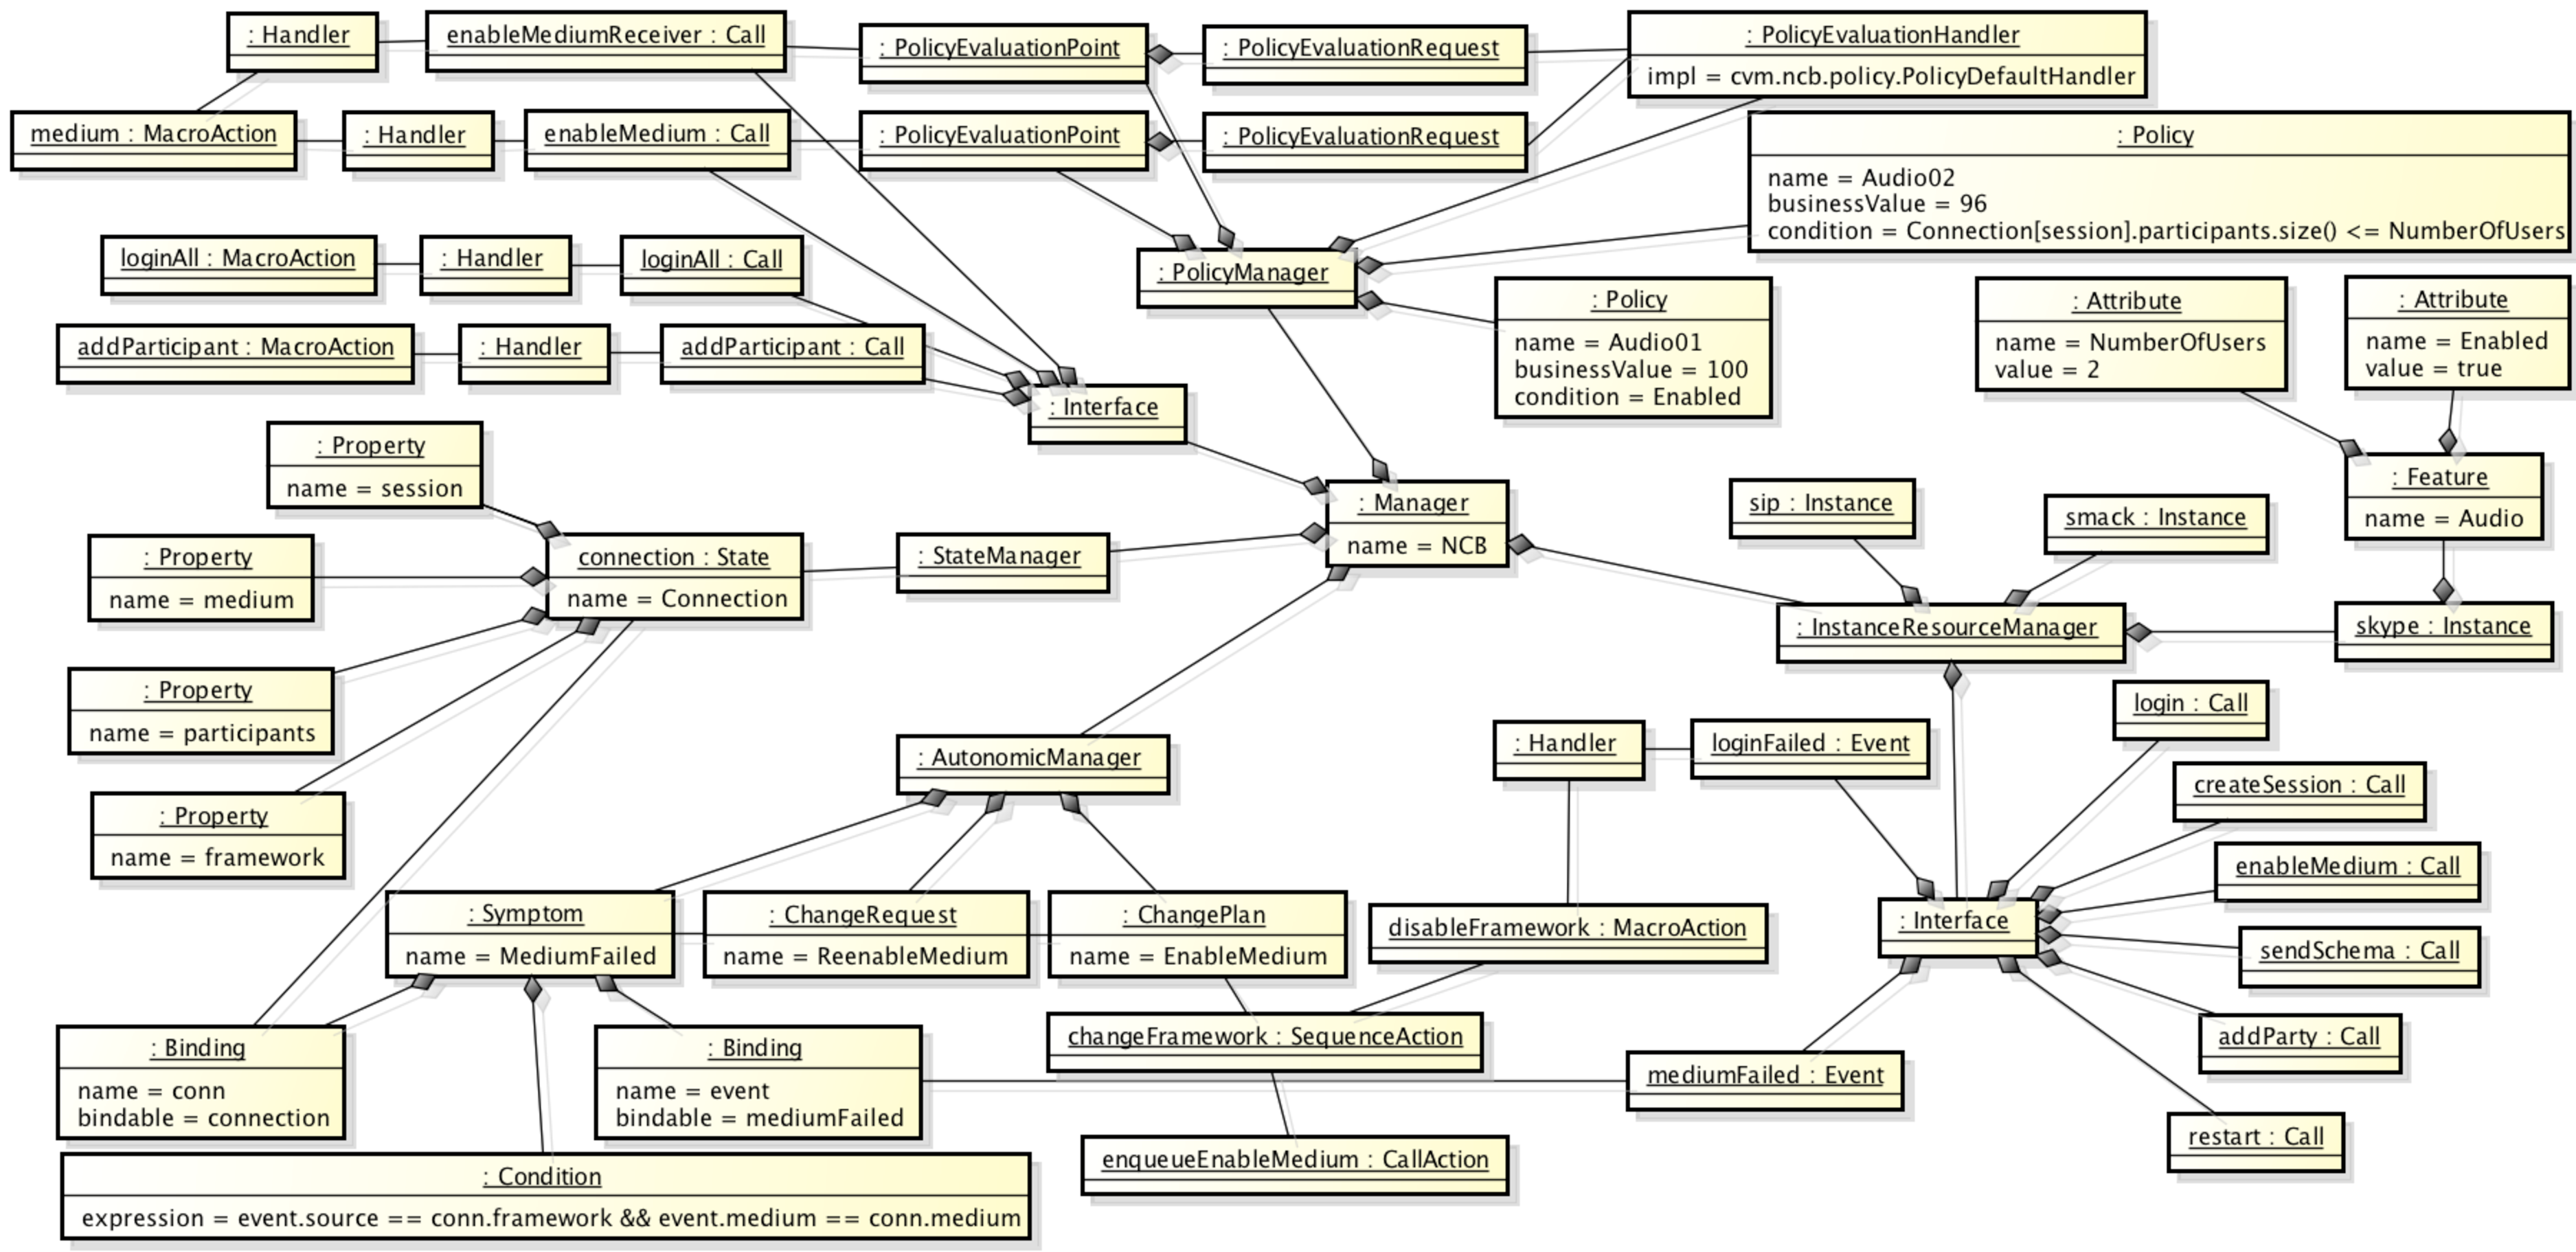
\includegraphics[width=0.9\textwidth]{instance}
 \caption{Instance of the broker layer  metamodel that describes a Network Communication Broker for the CVM}
 \label{fig:instance}
\end{figure*}


Figure ~\ref{fig:instance} shows an object diagram that illustrates a reduced part of the model designed. This diagram omits some relationships and objects due to space limitations. In this diagram, It is possible to outline how the main elements of the  metamodel are instantiated.


